\documentclass{article}
\usepackage{tikz}
\usetikzlibrary{matrix}

\begin{document}

\begin{center}
    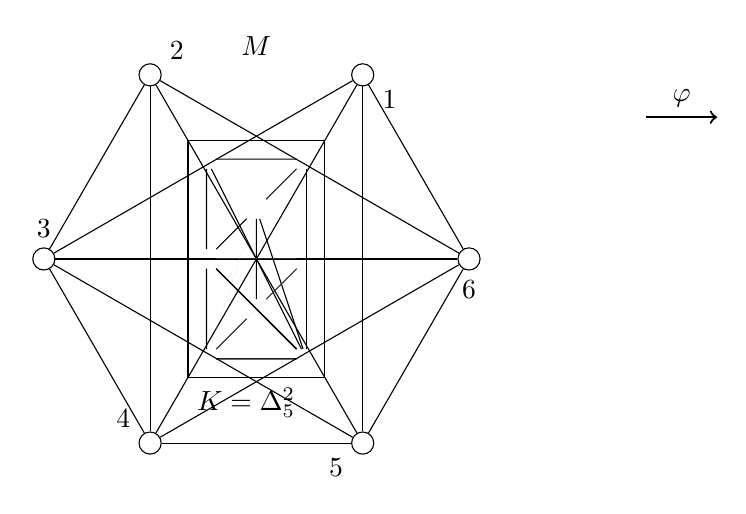
\begin{tikzpicture}[scale=0.9]
    
    % Define vertices for M
    \foreach \i in {1,...,6} {
        \node[circle,draw,inner sep=0pt,minimum size=8pt,label={270+\i*60}:$\i$] (v\i) at (\i*60:3) {};
    }
    
    % Connect vertices for M
    \foreach \from/\to in {1/3, 1/4, 1/5, 1/6, 2/3, 2/4, 2/5, 2/6, 3/4, 3/5, 3/6, 4/5, 4/6, 5/6} {
        \draw (v\from) -- (v\to);
    }
    
    % Define vertices for K = Delta_5^2
    \matrix[draw, matrix of nodes, nodes in empty cells, column sep=4mm, row sep=4mm] (K) {
      |(7)| &   & |(6)| \\
      & |(5)| & \\
      |(4)| & & |(3)| \\
      & |(2)| & \\
      |(1)| & & |(1')| \\
    };
    
    % Connect vertices for K
    \draw (7) -- (6) -- (5) -- (4) -- (3) -- (2) -- (1) -- (1');
    \draw (7) -- (4) -- (1') -- (7);
    \draw (6) -- (3) -- (1') -- (6);
    \draw (5) -- (2) -- (1') -- (5);
    \draw (4) -- (1) -- (1') -- (4);
    
    % Label K
    \node[below right] at (K.south west) {$K=\Delta_5^2$};
    
    % Arrow indicating the mapping
    \draw[->, thick] (5.5,2) -- node[above] {$\varphi$} (6.5,2);
    
    % Shading for M
    \fill[gray!50] (1)--(3)--(4)--cycle;
    \fill[gray!50] (1)--(5)--(6)--cycle;
    \fill[gray!50] (2)--(3)--(4)--cycle;
    
    % Label for M
    \node at (0,3) {$M$};
    
    \end{tikzpicture}
    
    An Euler cover $\varphi\colon M\to \Delta_5^{2}$ of the 2-skeleton of the 5-dimensional simplex $\Delta_5$, which has six vertices $1,2,3,4,5,6$, fifteen edges and twenty triangular faces. The pseudomanifold $M$ has six vertices, thirty edges and twenty triangular faces (including the unbounded face in this planar drawing). Vertices with the same labels are identified, so $M$ is a sphere with six pinchpoints. Note that the three shaded areas of $M$ map to three pairwise face-disjoint tetrahedron boundaries in $K$. The white triangles (including the unbounded region) map to the boundary of an octahedron in $K$. This decomposes $K$ as a face-disjoint union of four spheres (circlets).
\end{center}

\end{document}